\documentclass[9pt,twocolumn,twoside]{osajnl}
%% Please use 11pt if submitting to AOP
% \documentclass[11pt,twocolumn,twoside]{osajnl}
\usepackage{graphicx}% Include figure files
\usepackage{dcolumn}% Align table columns on decimal point
\usepackage{bm}% bold math
\usepackage{natbib}
\usepackage{physics}

\journal{optica} % Choose journal (ao, aop, josaa, josab, ol, optica, pr)

% See template introduction for guidance on setting shortarticle option
\setboolean{shortarticle}{true}
% true = letter / tutorial
% false = research / review article
\newcommand{\bea}{\begin{eqnarray}}
\newcommand{\eea}{\end{eqnarray}}

% (depending on journal).




\title{Optical detection of paramagnetic defects in a CVD-grown diamond using Nitrogen-Vacancy centers}

\author[1]{C. Pellet-Mary}
\author[1]{P. Huillery}
\author[1]{M. Perdriat}
\author[2]{A. Tallaire}
\author[1]{G. H\'etet} 

\affil[1]{Laboratoire de Physique de l'Ecole normale sup\'erieure, ENS, Universit\'e PSL, CNRS, Sorbonne Universit\'e, Universit\'e Paris-Diderot, Sorbonne Paris Cit\'e, Paris, France.}

\affil[*]{Corresponding author: gabriel.hetet@ens.fr}

%% To be edited by editor
% \dates{Compiled \today}

%\ociscodes{(140.3490) Lasers, distributed feedback; (060.2420) Fibers, polarization-maintaining;(060.3735) Fiber Bragg gratings.}

%% To be edited by editor
% \doi{\url{http://dx.doi.org/10.1364/XX.XX.XXXXXX}}

\begin{abstract}
The spins of Nitrogen Vacancy centers in Chemical Vapor Deposition (CVD) grown diamonds form ideal probes of magnetic fields and temperature, as well as ideal qu-bits for quantum information processing. 
Studying and controlling the magnetic environment of NV centers in such high purity crystals is thus essential.
In this letter, we demonstrate optical detection of paramagnetic species in a CVD grown diamond, such as hydrogen-related complexes, by coupling them to NV centers.
%We also unravel the role played by double quantum processes at zero magnetic field in the NV relaxation. 
The resonant transfer of NV centers spin-polarization to the electronic spins of these defects induces a loss of the NV photoluminescence, generating conspicuous features in the NV photoluminesence. 
The resonant condition is tuned with high accuracy by scanning a magnetic field along the 100 crystal direction.
Our results offer prospects for more detailed studies of CVD grown processes as well as for coherent control of the spin of a novel class of paramagnetic species.
\end{abstract}

\setboolean{displaycopyright}{true}

\begin{document}

\maketitle

\section{Introduction}
The electronic spin properties of the negatively charged nitrogen-vacancy (NV$^-$) center in diamond has given rise to a wealth of applications in nanoscale sensing and quantum information science. One major reason is that it can be optically polarized and read-out and features long coherence time even at ambient conditions. 
%The NV property can also then be employed to manipulate and to detect other dark spins that are interacting with it through dipole-dipole coupling, either inside or outside the diamond. 
In order to optimize the capabilities of the NV center, its magnetic environment must be controlled carefully. 
Synthetic growth of diamond crystal now reaches a level of control that makes pristine diamond crystals almost flawless, eliminating the source of magnetic noise from other nearby impurities. The standard growth technique works through Chemical Vapor Deposition (CVD) of carbon atoms from a methane gas in an ultra clean vacuum environment. It offers the possibility to work with 99.9\% purity as well as using 12C enriched methane, hence removing spin fluctuations fro 13C atoms. More results from CVD. 

The control of the purity of the material is typically done using Electron-Paramagnetic-Resonance (EPR). 
EPR operates with a very high resolution and was instrumental for detecting many species in diamond (uni of Warwick's review).
It would also be ideal if the defects were detected in the same platform that is used to for nanoscale sensing and quantum information processing, namely confocal microscopy. 
This would offer the opportunity to polarize these defects using the NV center, dynamically decouple them from the NV evolution for enhanced AC magnetometry and even to use them as ancilla qubits. 

 \begin{figure}[htbp]
\centering
\fbox{\includegraphics[width=\linewidth]{Fig1.eps}}
\caption{Schematics showing various paramagnetic defects in CVD grown diamonds polarized by a Nitrogen Vacancy center. Bottom right :  crystalline structure of the diamond.}
\label{fig1}
\end{figure}


%There has been a renewal of interest recently on the production of heavily doped diamonds recently.  
%Lukin, meyer....budker. 
%Cross relaxation amongst closely-packed NV centers can take place at moderate magnetic fields \cite{van_oort_optically_1991, van_oort_cross-relaxation_1989, armstrong_nvnv_2010, jarmola_longitudinal_2015, akhmedzhanov_microwave-free_2017, akhmedzhanov_magnetometry_2019, holliday_optical_1989, choi_depolarization_2017}, thus far, other impurities generally require by scanning large magnetic fields (more than hundreds of gauss) along the 111 direction of diamond. 
%This is generally required to probe paramagnetic impurities that have a small ZFS. 
%Most of the measurements are done at the ESLAC/GLSAC. OORT, BUDKER, HOLLENBERG, BAJAJ, MANSON.

%It is more difficult to obtain large concentration of Nitrogen-Vacancy centers in diamonds made from Chemical vapour deposition (CVD). 
%Cross-relaxation studies are more scarce using CVD doped diamonds.  

Here, we use confocal microscopy and a high-density NV ensembles in a CVD grown diamond to detect paramagnetic defects from CVD grown sample.
The detection was realized using cross-correlation studies through magnetic field scans. 
Cross-relaxation typically takes place when the electronic or nuclear spins of two atomic species exchange their polarization via resonant magnetic dipole-dipole interactions. 
If the spin of an NV center is polarized and coupled to an unpolarized spin B, it will lose part of its polarization at the expense of B and thus see a drop of its PL rate. 
Tuning the frequency of both spin transitions will thus result in a drop of the NV photoluminescence when that they are co-resonant, thus enabling detection of the spin state of B.

The hamiltonian that describes typical spin-1 defects in diamond under a magnetic field be written as 
\bea
\hat{H}=\hbar D S_z^2+\hbar \gamma_e\bm S \cdot \bm B
\eea
where $S$ is...
The first term describes dipole interactions amongst the two electrons of the spin-1 system. The second term describes the Zeeman interaction.
$D$ can vary significantly from one defect to another as it is sensitive to the local crystal field. It can then be used to find the structure of the defect in EPR measurements.
Also, hyperfine interactions can add zero-field splittings that can be observed under high resolution scans. 
The angle of the magnetic field can thus also be to bring defects into resonance. 

Cross relaxation amongst closely-packed NV centers can take place at moderate magnetic fields \cite{van_oort_optically_1991, van_oort_cross-relaxation_1989, armstrong_nvnv_2010, jarmola_longitudinal_2015, akhmedzhanov_microwave-free_2017, akhmedzhanov_magnetometry_2019, holliday_optical_1989, choi_depolarization_2017}, thus far, other impurities generally require by scanning large magnetic fields (more than hundreds of gauss) along the 111 direction of diamond. 
This is generally required to probe paramagnetic impurities that have a small ZFS. 
Most of the measurements are done at the ESLAC/GLSAC. OORT, BUDKER, HOLLENBERG, BAJAJ, MANSON.
Similar cross relaxation phenomena were studied by measuring changes in the optical hole depth in the zero-phonon line and studying decay rates oin stimulated spin-echo and spin-locking signals ? (BUDKER).

This procedure was proven useful for detecting the spin of $^{13}C$ atoms and the substitutional nitrogen Vacancy center in diamonds in the past. Such measurements not only show detection of this dark spins but can also be used to polarize them (Polarisation of 13C at low fields : PINES, MERILES ?). 
To date however, most studies have however been carried out using crystals grown by the High-Pressure-High-Temperature (HPHT) process, where a poor control over the paramagnetic defect density is available. In CVD grown samples, the typical paramagnetic impurities that have been detected by EPR are hydrogen complex such as the NVH, VH, VH2, where the hydrogen comes from the methane in the reactor. Fig.  \ref{fig1} shows a schematics of the various paramagnetic defects in a CVD grown diamonds that can be coupled to the Nitrogen Vacancy center in our study.

\begin{figure}[ht]
\centering
\fbox{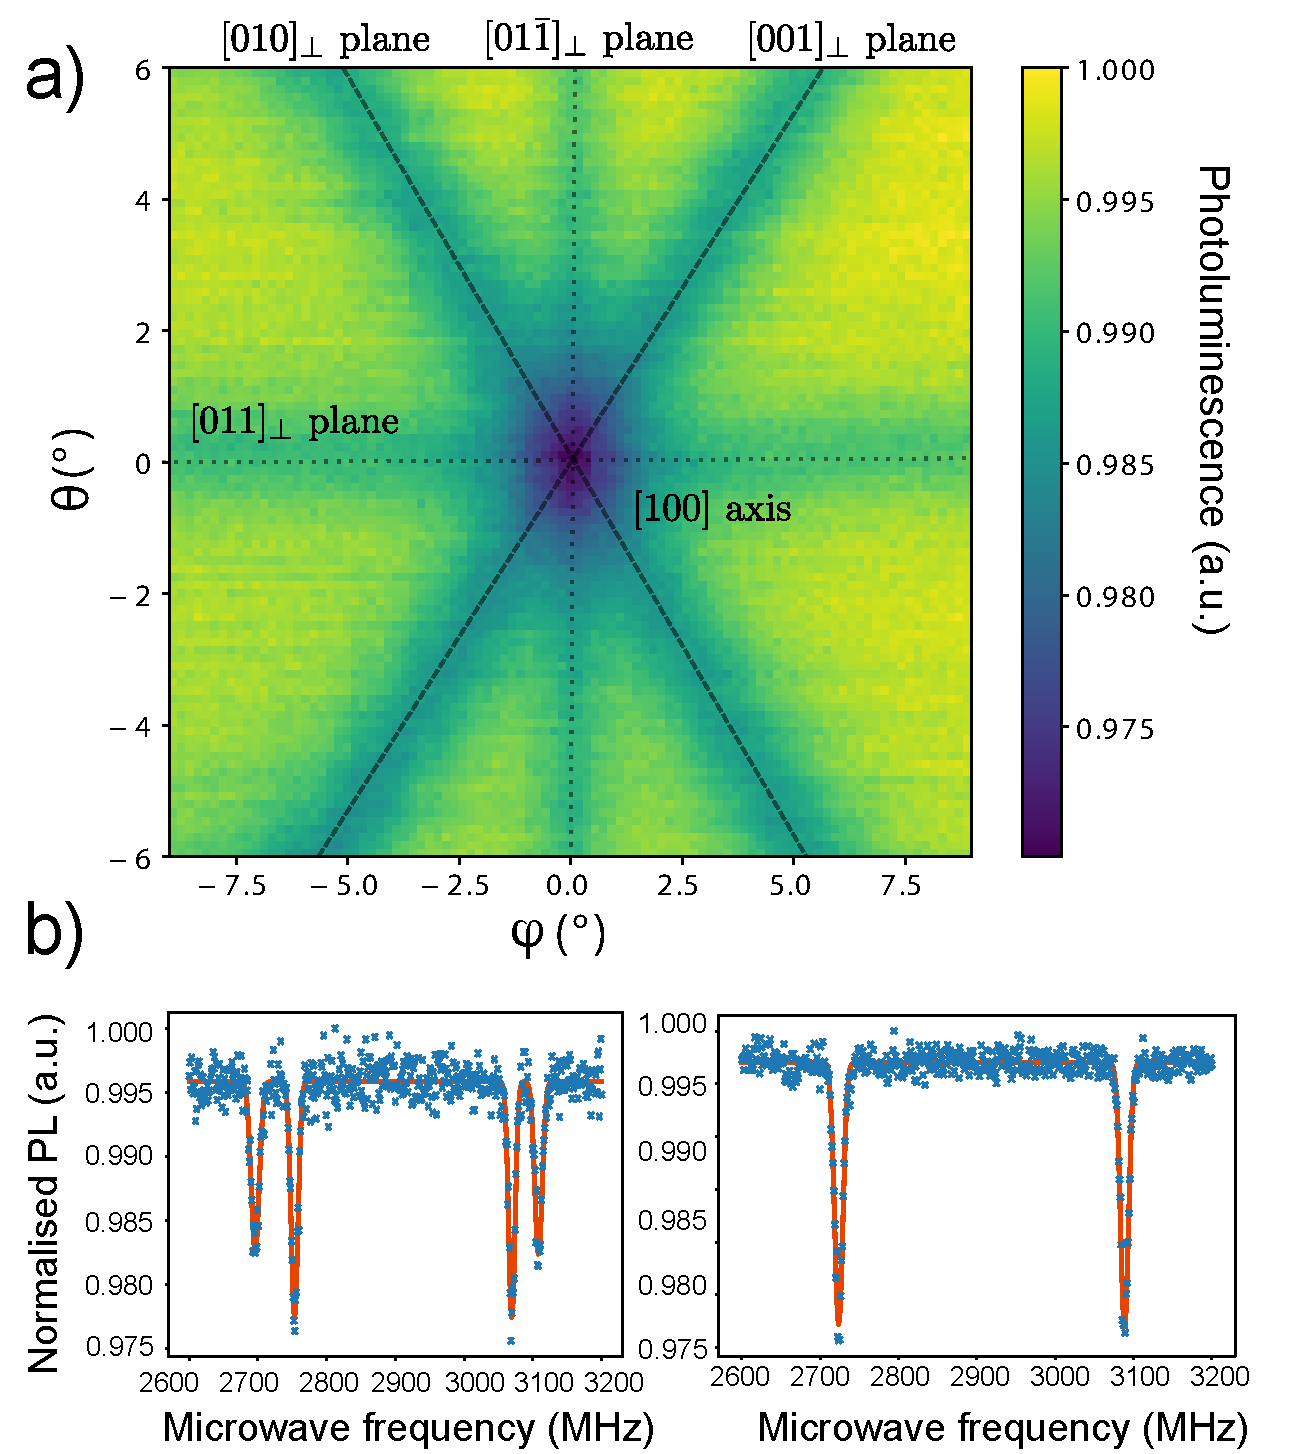
\includegraphics[width=\linewidth]{Carte_annotation}}
\caption{NV$^-$ photoluminescence as a function of a scanning magnetic field around the [100] crystalline directions with a fixed amplitude $|B|=115G$. The planes orthogonal to the [010],[001],[011], and [01$\bar 1$] directions are indicated by dashed lines.}
\label{map}
\end{figure}
 
Recent work in the doping processes has shown the possibility to reach NV centers concentrations in the 3 to 5 ppm range in CVD grown samples \cite{Edmonds, TALLAIRE2020421, MINDARAVA2020182}, without sacrificing the $T_2^*$ coherence time, opening a path towards detecting these hydrogen-related complexes using cross-relaxation with NV centers.
%Several impurities in CVD grown diamonds have been detected using Electron-Paramagnetic Resonance.  In order to purify diamond crystal and optimize their conduction and properties for prolonged qubit lifetimes. 
%Extensive work has been done in the past twenty years to detect and characterize the various  that appear in EPR. 
The sample we use in this study was grown using CVD with the addition of N$_2$0 in the methane phase. Then, high energy electron irradiation and in-situ annealing was realized in order to convert the nitrogen into NV centers. A concentration of 5 ppm of NV center was obtained.
It was shown that in this sample the $T_2^*$ was not degraded after annealing, and that the NV density was large enough to enable the observation of $T_1$ dependent concentration.  It is well-known that when the NV concentration increases above 1 ppm, the longitudinal decay of NV centers is degraded. 
Furthermore, it has been observed that cross-relaxation amongst closely pack NVs of different classes can be observed.
It was postulated that such a degradation of the $T_1$ time came from the coupling of NV centers to other NV related defects whose spin fluctuates. 
 
To perform the cross-relaxation detection, we use a homebuilt confocal microscope that comprises a 1mW green laser, an objective with a numerical aperture of XX to focus the laser onto the sample as well as to collect the PL. The PL was filtered from the green laser using a dichroic mirror and a notch filter coupled to a multimode fiber and sent to avalanche photodiode. The magnetic field scans were realized using a C-shaped electromagnet driven by a XX generator.  We monitor the NV PL as the magnetic field is scanned. 


Contrary the more commonly chosen $\langle 111 \rangle$ direction, we use magnetic field scans along the $\langle 100 \rangle$ direction. 
Looking at the diamond structure (bottom right in Fig.  \ref{fig1})-a), we see that in this direction, the four possible projections of the NV centers along the magnetic field are the same. This means that doing a B field scan along this direction will not make NV centers energies from different classes cross. At arbitrary angles, this can result is several lines that could mask cross-relaxation from other species. 
The down side of this choice of B field direction is that for large B field amplitudes, the transverse component of the B field makes the PL drop [], thus limiting the range of magnetic field amplitudes that can be employed.
In order to find the $\langle 100 \rangle$ direction we perform a preliminary angular scan of the magnetic field using a goniometer at a fix magnetic field amplitude.
Fig. \ref{map}-a)  shows the NV Photoluminescence as a function of magnetic field direction, referenced by azimuthal and polar angles $(\phi, \theta)$ in the above described CVD grown sample. The PL is seen to drop for particular values of the angle as anticipated.
%The symmetric pattern suggests that the diamond crystalline main directions play a role. Because of the anisotropy of the NV center, see \ref{Cristallo}, the NV PL drop can indeed be a signature of the crystal direction.
Such a drop of the PL along the crystal axis was already observed by many groups. LUKIN, HEMMER, BUDKER. JARMOLA. OORT
\cite{van_oort_optically_1991, van_oort_cross-relaxation_1989, armstrong_nvnv_2010, jarmola_longitudinal_2015, akhmedzhanov_microwave-free_2017, akhmedzhanov_magnetometry_2019, holliday_optical_1989, choi_depolarization_2017} and correspond to situation where NV centers cross. 
Using such a map enables to identify clearly the crystalline axis and, in particular, the central point on this map, the $\langle 100 \rangle$ direction.

The planes orthogonal to the [010],[001],[011], and [01$\bar 1$] directions are indicated by dashed lines and show the locus of the cross relaxation, with a smaller PL contrast. 
The width of the CR peak is compatible with the $T_2^*$ time at this B field values. The contrast is determined both by the fluctuating NV concentration and the polarized NVs.
Such a map can in itself be a useful tool in order to measure magnetic fields without microwave, as already pointed out in \cite{}. 

To double check these interpretations, we run an electron spin resonances by fixing the magnetic field amplitude and by scanning the microwave frequency. 
Fig. \ref{map}-b) shows an ESR taken at the angle ... showing two degeneracies.
Fig. \ref{map}-b) shows an ESR taken at the angle .. .showing four degeneracies. This hints towards the 100 direction. 

We now tune the magnetic field along the 100 direction and scan the magnetic field amplitude. 
Fig. \ref{scan} shows the PL as a function of magnetic field amplitude, along the $\langle 100 \rangle$ direction in the 15 G to 145 G range. 
Careful calibration of the magnetic field amplitude was realized using a microwave tone of known frequency ....
The angle was controlled to within XX. 
For these data, the averaging was done for XX days. 
Three features clearly appear in this spectrum : one broader feature at 20G, another one at 56 G and one last one at 122 G. 
We also note an overall drop of the PL, as a the result of state mixing in the optically excited state. 
We made attempts to fit this curve using the full 7 level model, but this only gave poor agreement with experimental data. Further work will be done in order to clarify this. 
In order to let the three salient features detach better from the spectrum, we thus resorted to a 4th order polynomial fit without the spectral bumps, and subtract it from the curve. The subtracted curve is displayed below.  The width and contrast of each peak can now be compared and the position of each peak can be determined with great accuracy. 

\begin{figure}[htbp]
\centering
\fbox{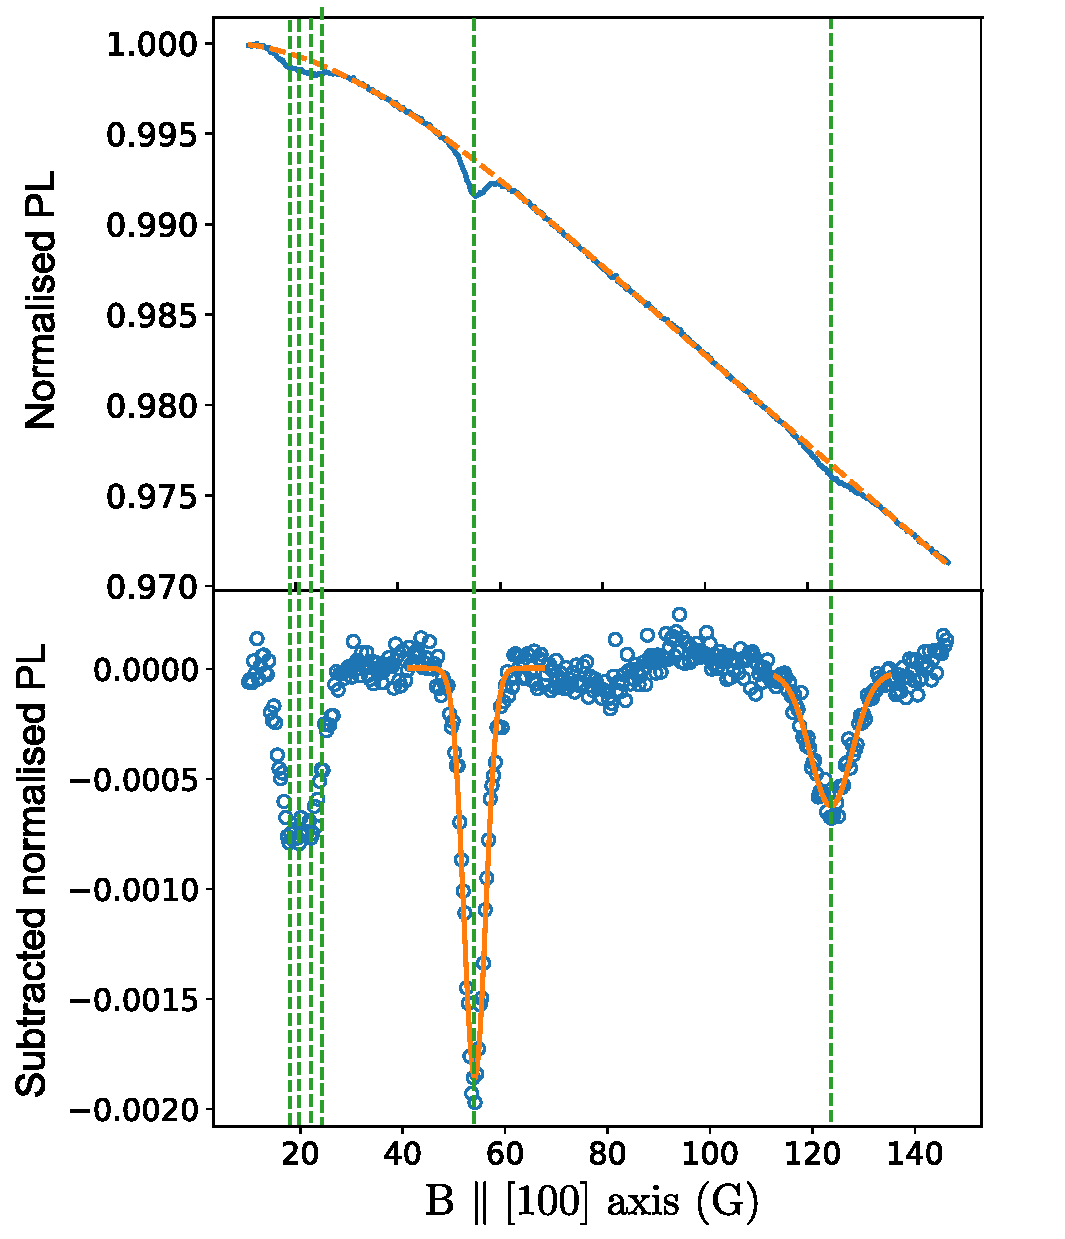
\includegraphics[width=\linewidth]{Scans_fig4}}
\caption{Optical detection of cross-relaxations. \textbf{Top} NV$^-$ photoluminescence while scanning the magnetic field along the [100] crystalline direction (plain line) and polynomial fit to the fourth order (dashed line). \textbf{Bottom} Subtraction of the previous signal by the polynomial fit (circles), simulated CR magnetic field amplitude (dashed,vertical) and gaussian fits for the second and third dips (plain line)}
\label{scan}
\end{figure}

In order to attribute the the three features to their respective defects, we run a similar scan (not shown) on heavily doped HPHT diamond samples in the same 100 direction. Only the first feature appeared. 
This observation led us to search for CVD specific defects as candidates for the last two peaks. Paramagnetic defects in CVD grown diamonds have been extensively studied using EPR at the university of Warwick. These studies demonstrate that  NVH, VH, VH2 complexes can be stable in diamond and they also estimate the zero-field splitting $D$ for most of them.
Oxygen related complex may also occur here, due to our N2O are not resonant (https://core.ac.uk/download/pdf/46556.pdf)
The first peak could then be coming from dipolar coupling between NVs and paramagnetic defects that are present in all diamonds, such as the substitutional nitrogen, also called $P_1$ centers ($[P_1]\approx 10 ppm$ ?) and the ${13}^C$ atoms (${13}^C= 1\%$). 
Using the results from Budker et al. we first intended to correlate the peaks with NV centers that are coupled to $P_1$ centers. 
 $P_1$ centers have a small zero-field splitting so in order to appear a such small magnetic fields, they would first have to be coupled to an NV centers and then be coupled to a nearby polarized NV.
The obtained eigenfrequencies were inconsistent with our observed peaks and our spectral resolution error (~1G). This lead us to consider the ${13}^C$ atoms. 
In itself, the ${13}^C$ spin has a very small zero-field splitting too (=?). In order to give a contribution to the spectra, it would have to be strongly coupled to an NV center. 
In this case, the $^{13}$C-NV pair would show 4 transitions corresponding to ....

Fig. \ref{energy-levels} shows the transition frequencies of the NV$^-$, the $^{13}$C-NV pair and the VH- as a function of the magnetic field amplitude along the 100 direction.
The energy evolution of another defect, whose structure is unknown, and was coined the WAR1 defects is plotted on this graph. 
The points were the NV levels cross the other defects would in principle correspond to an enhanced double quantum cross-relaxation process between the NV and the presumably unpolarized species. 
The NV0 ?


\begin{figure}[htbp]
\centering
\fbox{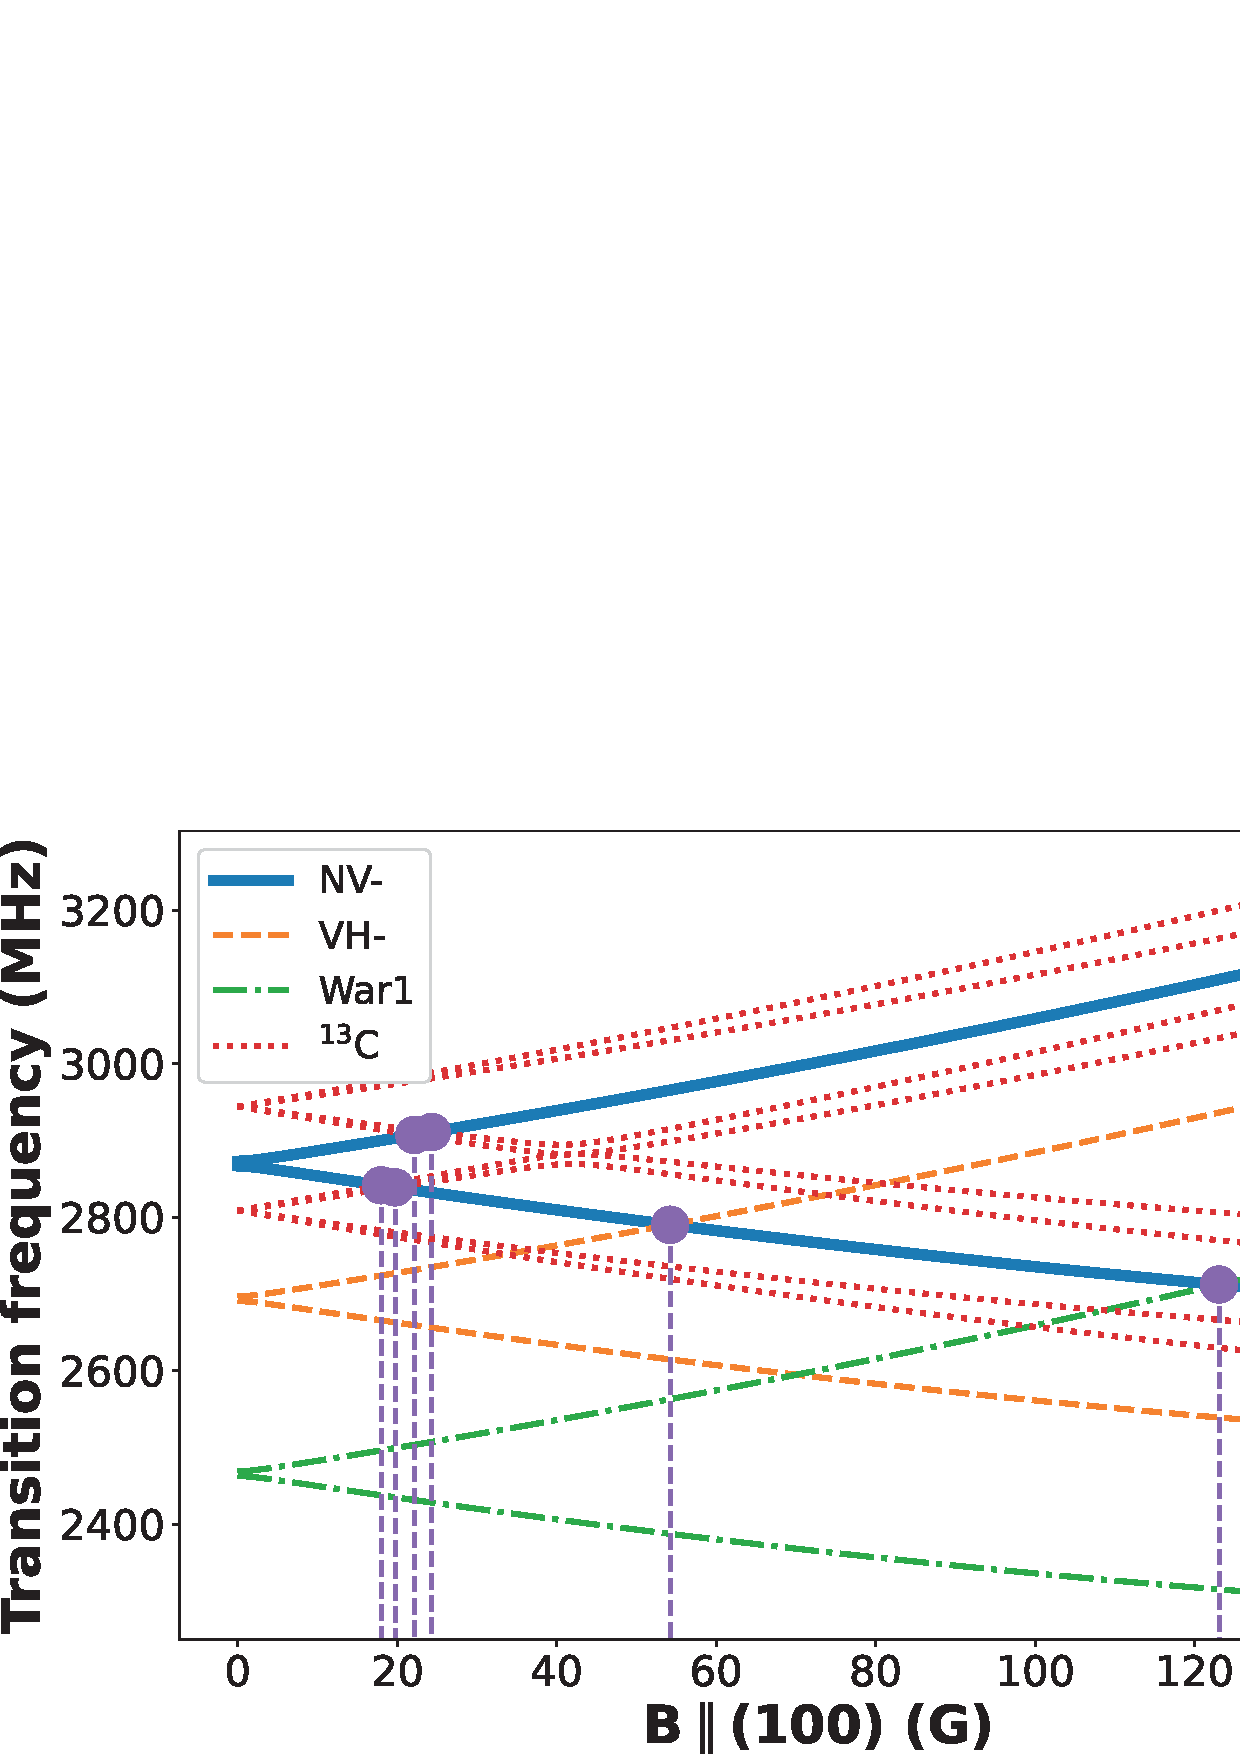
\includegraphics[width=\linewidth]{Theorie_CR}}
\caption{Simulated transitions energies of the various spins considered as a function of a magnetic field aligned along the [100] axis. NV centers transitions are represented using a plain line, VH$^-$ using a dashed line, the WAR1 using a dash-dotted line and $^{13}$C-NV pair using a dotted line. The amplitudes of the magnetic field where the energy level of the NV center crosses the one of another species are represented by vertical dashed lines}
\label{energy-levels}
\end{figure}


The first peak that we observe coincides with cross-relaxation that is expected to take place with $^{13}$C atoms that is one shell away from the Nitrogen vacancy centers. 
This drop of the PL is consistent with $^{13}$C-NV pair.  Using typical values found in the literature for the unpolarized NVs (also called fluctuators), we can estimate the concentration of this $^{13}$C-NV pair to be XX, making this hypothesis very likely. 
The second peak that we observe coincides very well with the crossing between the 0 to -1 NV transition and the 0 to +1 VH- transition.
Such a defect was studied in details in XXX and was found to have a $D=$. 
Making a gaussian fit to this data show that the position of the detected peak is , which gives a $D=$.
Estimation suggest that the concentration of this defect is about 100 ppb (?).

The third peak corresponds to a spin defect that has a D=.
We found in Cruddace that it was already observed in EPR, although its structure is unknown.



NVH (H3) center (diamagnetic in ground state), paramagnetic only in excited state but requires UV light. 
No other species were observed in the optical spectrum or EPR. 



The technique can be used to detect the degree of polarisation of $^{13}$C atoms at room temperature.


Table \ref{tab:shape-functions} 


\begin{table}[htbp]
\centering
\caption{\bf Zero-field splitting parameter $D_z$ for the different spin-1 species}
\begin{tabular}{ccc}
\hline
$D_z$ estimation (MHz) & Cruddace's work\citep{cruddace2007magnetic} & Our work \\
\hline
NV$^-$ & 2872(7) & * \\
VH$^-$ & 2706(30) & 2694(5)  \\
WAR1 & 2466(60) & 2470(10) \\
\hline
\end{tabular}
  \label{tab:shape-functions}
\end{table}



\section{Funding}
GH acknowledges funding by the French National Research Agency (ANR) through the T-ERC project QUOVADIS. 

\section{Acknowledgments}
We would like to thank Neil Manson and Carols Meriles for fruitful discussions. 





\section{Disclosures}

The authors declare no conflicts of interest.'

% Bibliography
\bibliography{Biblio_CVD-CR}

% Full bibliography added automatically for Optics Letters submissions; the following line will simply be ignored if submitting to other journals.
% Note that this extra page will not count against page length
\bibliographyfullrefs{sample}




\end{document}
